\section{The 8259 Interface Chip}

\subsection{Background}

8259 microprocessor is defined as \textit{Programmable Interrupt Controller (PIC)}  microprocessor.
There are 5 hardware interrupts and 2 hardware interrupts in 8085 and 8086 respectively. But by
connecting 8259 with CPU, we can increase the Interrupt handling capability. 8259 combines the
multi-interrupt input sources into a single interrupt output. Interfacing of single PIC provides 8
interrupts inputs from \textit{IR0-IR7}.

For example, interfacing of 8085 and 8259 increases the interrupt handling capability of 8085
microprocessor from 5 to 8 interrupt levels.

\subsection{Features of 8259}

\begin{itemize}
    \item Intel 8259 is designed for Intel 8085 and Intel 8086 microprocessor.
    \item It can be programmed either in level triggered or in edge triggered interrupt level.
    \item We can mask individual bits of interrupt request register.
    \item We can increase interrupt handling capability up to 64 interrupt level by cascading
          further 8259 PIC.
    \item Clock cycle is not required
    \item It can be programmed in 8085 and 8086 microprocessor.
\end{itemize}

\subsection{Pin Description}

\begin{figure}[ht]
    \centering
    
\includegraphics[width=0.4\textwidth]{res/practicals/8259pins.png}
    \caption{Pin Diagram of 8259}
    \label{fig:8259_pin}
\end{figure}

\subsection{Block Diagram}

\begin{figure}[ht]
    \centering
    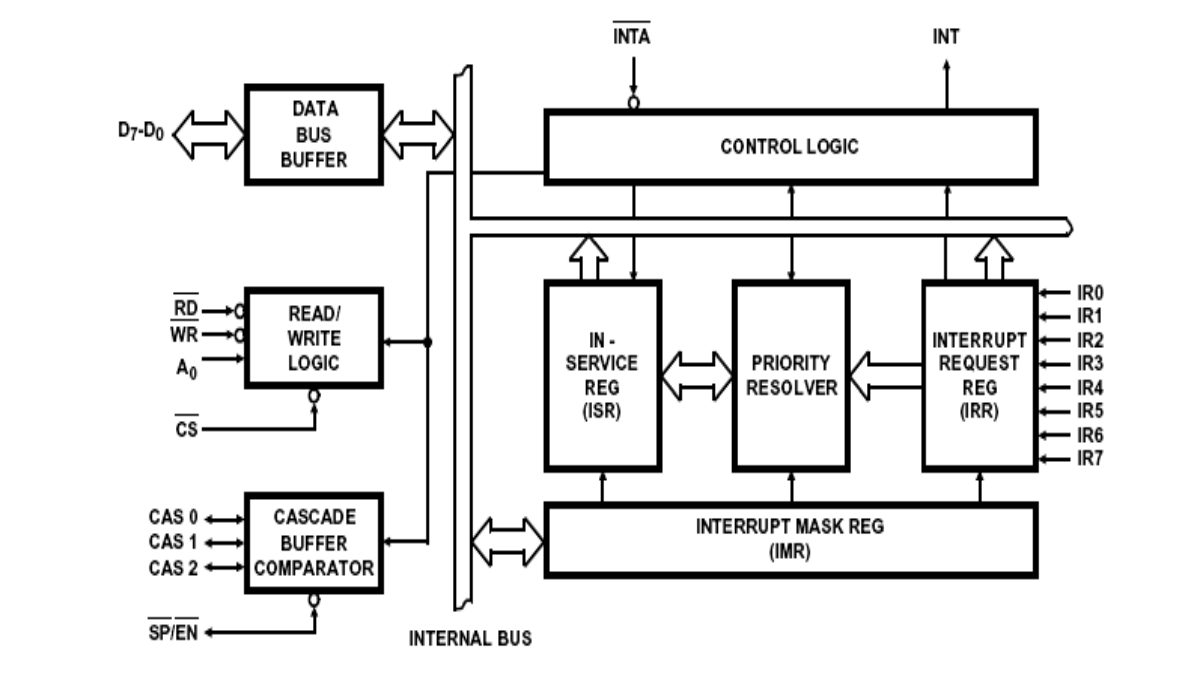
\includegraphics[width=0.9\textwidth]{res/practicals/8259.png}
    \caption{Block Diagram of 8259}
    \label{fig:8259}
\end{figure}

The block diagram consists of 8 blocks which are:

\begin{itemize}
    \item  Data bus buffer
    \item Read/Write Logic
    \item Cascade Buffer Comparator
    \item Control Logic
    \item Priority Resolve
    \item Interrupt Request Register (IRR)
    \item Interrupt Service Register (ISR)
\end{itemize}